% Oppsett, ikke noe å bry seg om.
\documentclass[12pt,norsk,a4paper]{article}
\usepackage{graphicx}
\usepackage{hyperref}
\usepackage{float}
\usepackage{pdfpages}
\usepackage{ulem}
\usepackage[utf8]{inputenc}
\usepackage[norsk]{babel}
\usepackage{multirow}
\usepackage{colortbl}
\usepackage{array}

\begin {document}
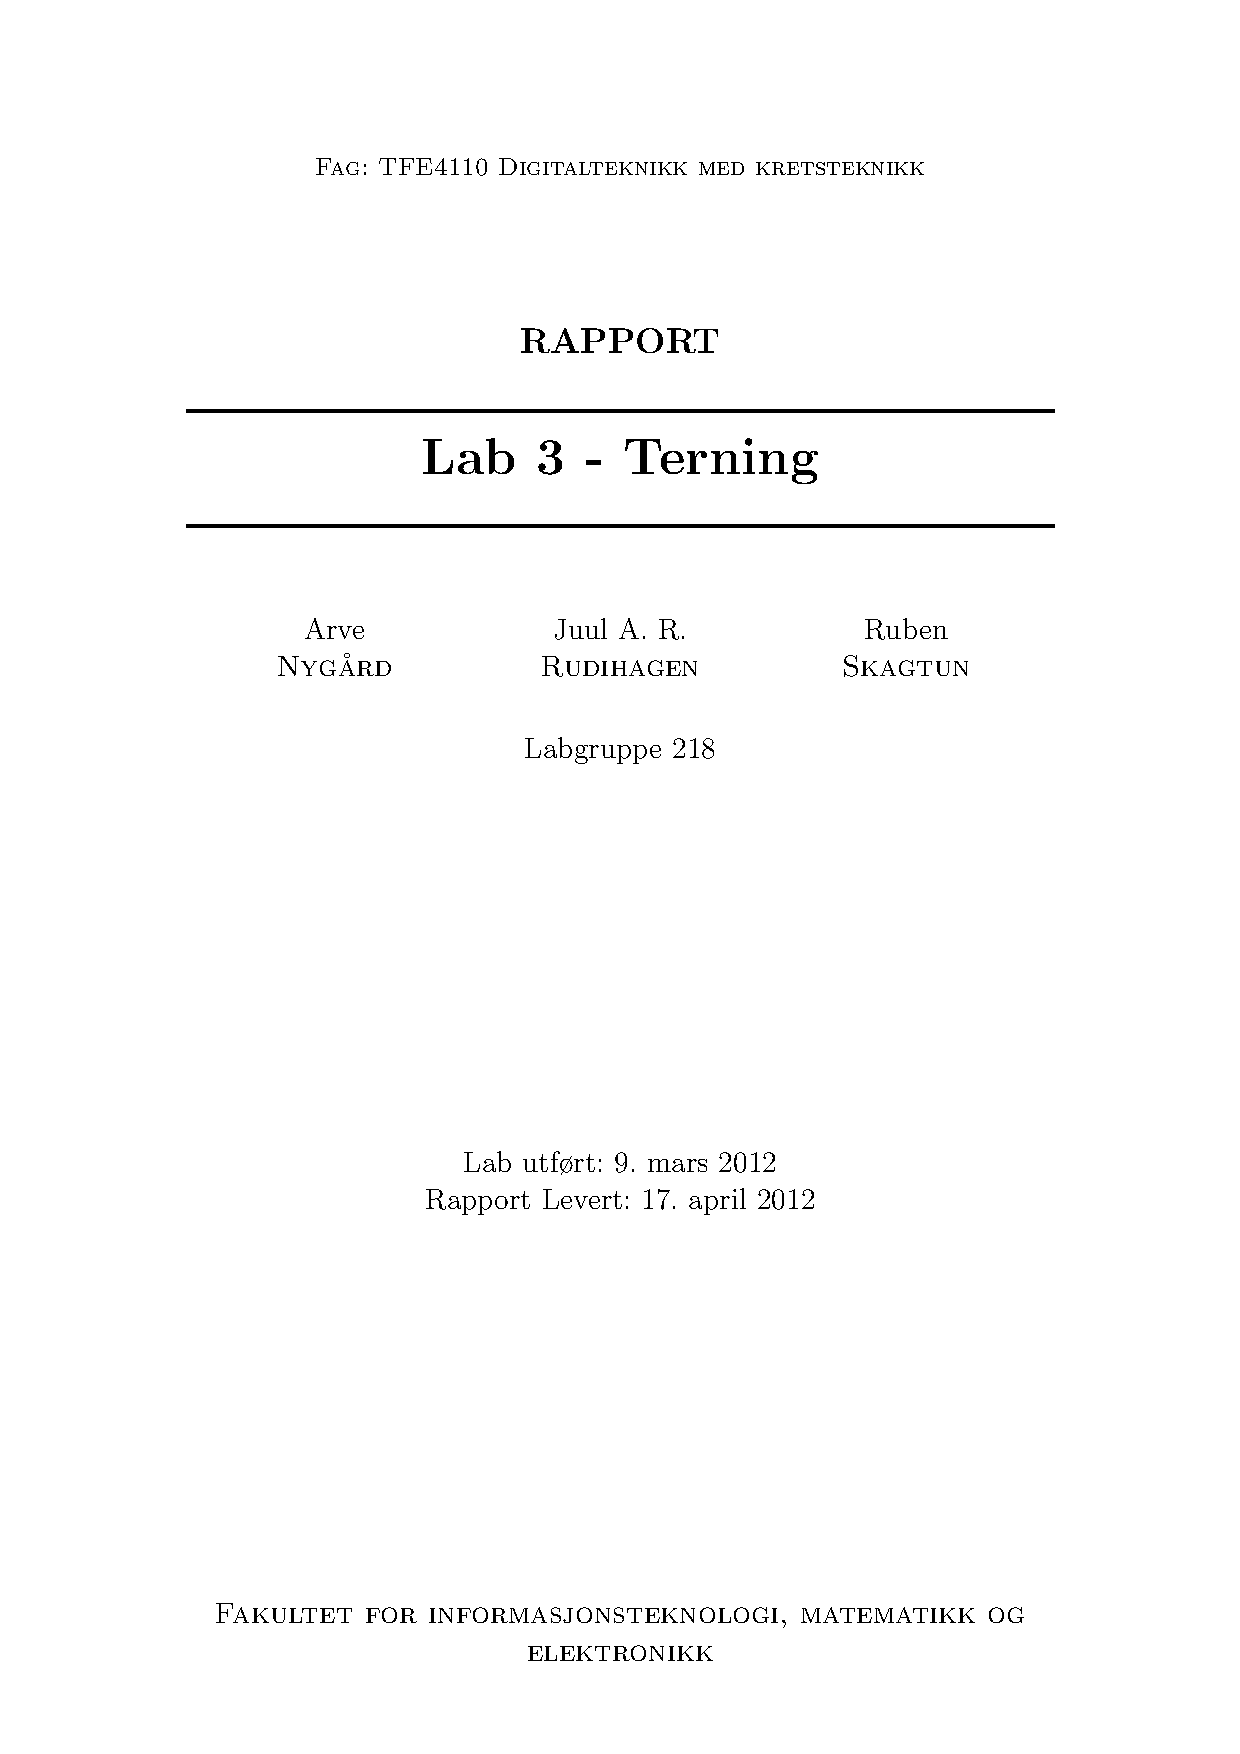
\includepdf{titlepage}
\clearpage



\section*{} % Stjerne etter section -> Siden tas ikke med når latex teller sidetall
\thispagestyle{empty}   
\begin{center}
\Large \textsc{Labrapport: Lab 3 - Terning}
\end{center}
\clearpage

\section*{Sammendrag}
\thispagestyle{empty}  
I denne rapporten blir det beskrevet hvordan gruppen utførte en laboppgave hvor målet var å lage en digital krets, ved hjelp av diskrete portkretser, som styrer lysdioder slik at de danner mønstrene til en vanlig sekssidet terning. Et viktig poeng er at terningen skal ha en uniform verdidistribusjon, slik at den oppfører seg som en virkelig terning.

Etter å ha kommet frem til et design på papiret, ble kretsene loddet opp og testet. Gruppen fikk produsert to kretser som viste tilfeldige terningmønstre, som etter 60 testkjøringer viste seg å ha en uniform distribusjon av verdier. Et tredje kretskort ble startet på, men ikke fullført i tide.
\clearpage

\tableofcontents %Innholdsfortegnelse. Genereres automatisk. :)
\thispagestyle{empty}   
\clearpage

\section{Innledning} 
\setcounter{page}{1}
INNLEDNING\
skriv her
\clearpage

\section{Teoretisk grunnlag}
Terningen består av tre hoveddeler som vi skal forklare hvordan fungerer. Det er en tilfeldig tallgenerator som til enhver tid
gir ut et trebits binærtall mellom 001 og 110, som er henholdsvis 1 og 6. Logikken skal så oversette denne tallrekken til et nytt firebits binærmønster som styrer lysdiodene. Til slutt er lysdiodene som lyser et tall mellom en og seks som vist på en terning. Se figur under:
\begin{figure}[H]
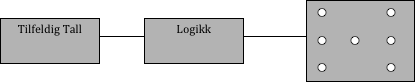
\includegraphics{Blokkskjema.png}
\caption{Hoveddelene til terningen}
\label{fig:blokkskjema}
\end{figure}

    \subsection{Tilfeldig tallgenerator}
    Den tilfeldige tallgeneratoren baser en teller som teller fra 1 til 6 i en evig loop. Dette skjer vet at når telleren overstiger verdien seks begynner den å telle på en igjen. Telleren blir klokket av en oscillator som svinger
    veldig raskt, dette gjør at verdien til telleren skifter så fort at vi kan si det er tilfeldig hvilket tall som kommer ut når man slipper bryteren. Denne oscillatoren består av en NAND- og en NOR-port, i tillegg til noen motstandere og kondensatorer. Se figur under:
    \\
    \\
    \textbf{Her burde vi kanskje ha et bilde?} 

    
    \subsection{Lysdioder}
    Lysdiodene på kretskortet som vi bruker til å vise hvilket tall terningen får er aktiv lave. Det vil si at dersom de får inn '0'
    så vil de lyse. Selv om dette kan virke forvirrende er det hensiktsmessig fordi det fører til at vi får mindre indre motstand. Dette fører igjen til at vi får mer strøm som gir sterkere lys. For å gi ut alle tallene en terning kan gi, ved en mest mulig lik tilnærming trenger vi 7 lysdioder og 4 styresignal. Grunnen til at vi bare trenger 4 styresignal til 7 lysdioder er fordi noen av dem kan kontroleres med samme styresignal. Hvilket dioder som lyser samtidig er markert på figuren under:

    \begin{figure}[H]
    \begin{center}
    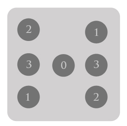
\includegraphics[scale=1]{Terning.png}
    \caption{Figur av terninen. Diodene med samme nummer lyser alltid samtidig}
    \label{fig:terning}
    \end{center}
    \end{figure}

    \subsection{Logikkken}
    Logikken sin oppgave er å oversette signalene Q2-Q0 som representerer den binære verdien til hvilket tall terningen skal gi, til styresignalene S3-S0 som styrer lysene på terningen. Et poeng er å gjøre kretsen så effektiv som mulig, for å oppnå dette brukte vi Karnaugh-Diagram. Utledningen som ble gjørt er lagt ved som Vedlegg 1 og Vedlegg 2. En kort oppsumering av resultatet vises i tabellen under.

    \begin{table}[H] 
    \begin{center}
        \begin{tabular}{ | c | l |} 
        \hline
        $Styresignal$  & $Logisk uttrykk$ \\ \hline 
        S0 & $\neg Q_0$\\ \hline
        S1 & $\neg Q_2 \wedge \neg Q_1$\\ \hline
        S2 & $\neg Q_2$\\ \hline
        S3 & $\neg Q_2 + \neg Q_1$\\ \hline
        \hline
        \end{tabular}
        \end{center}
        \caption{Tabell på hvordan logikken konverterer ingangsbittene til styresignalene}

\end{table}

    Ut fra denne tabellen kan vi sette opp hvordan den totale kretsen skal bli når vi kobler den sammen. Resultatet er fremstil på bilde under: 

    \begin{figure}[H]
    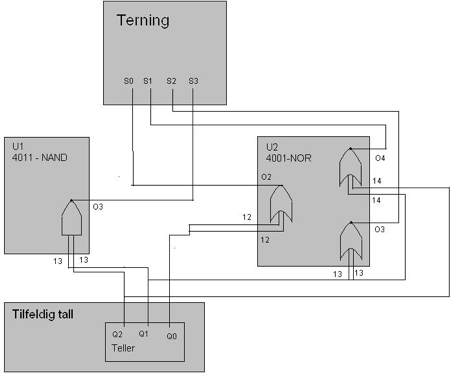
\includegraphics[scale=0.75]{Krestkortet.png}
    \caption{Sammenhengen mellom bitverdiene og styresignalende}
    \label{fig:krestkortet}
    \end{figure}

    Som en ser på bilde har vi lagd inverterere ved å koble samme inngangsignal i begge inngangene på en NAND- eller NOR-port. Vi kunne oppnådd samme effekt dersom vi koblet en av inngangene til jord.    

\clearpage

\section{Målemetode og arbeidsbeskrivelse}
\clearpage


\section{Utstyrsliste} 
    \begin{itemize} %Punktliste
    \item liste     %Punkt i listen
    \item for
    \item eksempel
    \end{itemize}
\clearpage


\section{Resultater}

Heiheihei
LOLOL
LOLOL
det var en gang en \textit{kursiv gris} og en  \textbf{bold ulv}
\subsection{Egen subsection for hver oppgavedel}


\begin{table}[H] %Eksempel på tabell.
\begin{center}
	\begin{tabular}{ | r | c |} %Tegn opp kolonner med bar ( | ), og ha r/c/l for right/center/left tekts-justering i tilsvarende kollonn
	\hline
	$X(cm )\pm0,2cm$  &$B(mT)\pm(0,3mT+1\%$) \\ \hline %$formel$ inline "mattemodus" - når du ikke gidder \begin{equation} osv.
    1 & 0,95\\ \hline   % \hline -> horizontal line -> ny linje i tabellen
    2 & 0,84\\ \hline
    3 & 0,71\\ \hline
    4 & 0,64\\ \hline
    5 & 0,54\\ \hline
    10 & 0,21\\ \hline
    15 & 0,09\\ \hline
    20 & 0,03\\ \hline
    30 & 0,00\\ \hline
    \hline
    \end{tabular}
    \end{center}
    \caption{Eksempel på tabell}

\end{table}
\clearpage

\section{Diskusjon}
\clearpage

\section{Konklusjon}
        \begin{equation} %Eksempel på likning. Denne får (1) bak seg.
            \label{eq:magnetfelt-spole} %Label lar deg referere til likningen.
            B(x) = \frac{\mu_0 N I}{2R} \Bigg(1 + \frac{x^2}{R^2} \Bigg) 
        \end{equation}
\clearpage

\section{Vedlegg}
    \subsection{Vedlegg 1 sammenheng mellom binærverdi og styresignal. ARVE FIKS DEN DRITTEN SOM STIKKER UT AV TABELLEN ER DU SNILL :P}
    \begin{table}[H]
    \begin{center}
    \begin{tabular}{|c|c|c|c|c|c|c|c|c|}
    \hline
    Hex & \multicolumn{3}{|c|}{Binærverdi} & \multicolumn{4}{|c|}{Styresignal}&hex \\ \hline
    $Q$ & $Q_2$ & $Q_1$ & $Q_0$ & $S_3$ & $S_2$ & $S_1$ & $S_0$ & $S$ \\ \hline
    0 & 0 & 0 & 0 & X & X & X & X & - \\ \hline 
    1 & 0 & 0 & 1 & 1 & 1 & 1 & 0 & E \\ \hline
    2 & 0 & 1 & 0 & 1 & 1 & 0 & 1 & D \\ \hline
    3 & 0 & 1 & 1 & 1 & 1 & 0 & 0 & C \\ \hline
    4 & 1 & 0 & 0 & 1 & 0 & 0 & 1 & 9 \\ \hline
    5 & 1 & 0 & 1 & 1 & 0 & 0 & 0 & 8 \\ \hline
    6 & 1 & 1 & 0 & 0 & 0 & 0 & 1 & 1 \\ \hline
    7 & 1 & 1 & 1 & X & X & X & X & - \\ \hline
    \end{tabular}
    \end{center}
    \caption{Resultat $S_0=\neg Q_0$}
    \end{table}

    \subsection{Vedlegg 2 Karnaugh-Diagram}
    \begin{table}[H]
    \begin{center}
    \begin{tabular}{|l|l|r|r|} \hline
    \multicolumn{4}{|c|}{Tabell for $S_0$} \\ \hline
    $Q_2$ & $Q_1$ & \multicolumn{2}{|r|}{$Q_0$ \hspace{20 mm} 0 \hspace{2 mm} 1} \\ \hline
    0 & 0 & \hspace{27 mm} X \cellcolor[gray]{0.8} & 0 \\ \hline 
    0 & 1 & 1 \cellcolor[gray]{0.8} & 0 \\ \hline
    1 & 1 & 1 \cellcolor[gray]{0.8} & X \\ \hline
    1 & 0 & 1 \cellcolor[gray]{0.8} & 0 \\ \hline
    \end{tabular}
    \end{center}
    \caption{Resultat $S_0=\neg Q_0$}
    \end{table}


    \begin{table}[H]
    \begin{center}
    \begin{tabular}{|l|l|r|r|} \hline
    \multicolumn{4}{|c|}{Tabell for $S_1$} \\ \hline
    $Q_2$ & $Q_1$ & \multicolumn{2}{|r|}{$Q_0$ \hspace{20 mm} 0 \hspace{2 mm} 1} \\ \hline
    0 & 0 & \hspace{27 mm} X \cellcolor[gray]{0.8} & \cellcolor[gray]{0.8} 1 \\ \hline 
    0 & 1 & 0 & 0 \\ \hline
    1 & 1 & 0 & X \\ \hline
    1 & 0 & 0 & 0 \\ \hline
    \end{tabular}
    \end{center}
    \caption{Resultat $S_1=\neg Q_2 \wedge \neg Q_1$}
    \end{table}


    \begin{table}[H]
    \begin{center}
    \begin{tabular}{|l|l|r|r|} \hline
    \multicolumn{4}{|c|}{Tabell for $S_2$} \\ \hline
    $Q_2$ & $Q_1$ & \multicolumn{2}{|r|}{$Q_0$ \hspace{20 mm} 0 \hspace{2 mm} 1} \\ \hline
    0 & 0 & \hspace{27 mm} X \cellcolor[gray]{0.8} & \cellcolor[gray]{0.8} 1 \\ \hline 
    0 & 1 & 1 \cellcolor[gray]{0.8} & 1 \cellcolor[gray]{0.8} \\ \hline
    1 & 1 & 0 & X \\ \hline
    1 & 0 & 0 & 0 \\ \hline
    \end{tabular}
    \end{center}
    \caption{Resultat $S_2=\neg Q_2$}
    \end{table}

    \begin{table}[H]
    \begin{center}
    \begin{tabular}{|l|l|r|r|} \hline
    \multicolumn{4}{|c|}{Tabell for $S_0$} \\ \hline
    $Q_2$ & $Q_1$ & \multicolumn{2}{|r|}{$Q_0$ \hspace{20 mm} 0 \hspace{2 mm} 1} \\ \hline
    0 & 0 & \hspace{27 mm} X \cellcolor[gray]{0.8} & \cellcolor[gray]{0.8} 1 \\ \hline 
    0 & 1 & 1 \cellcolor[gray]{0.8} & 1 \cellcolor[gray]{0.8} \\ \hline
    1 & 1 & 0 & X \\ \hline
    1 & 0 & 1 \cellcolor[gray]{0.8} & 1 \cellcolor[gray]{0.8} \\ \hline
    \end{tabular}
    \end{center}
    \caption{Resultat $S_3=\neg Q_2 + \neg Q_1$}
    \end{table}

\clearpage

\section{Litteraturhenvisninger}
\clearpage

\section{Tilbakemeldinger}
\clearpage
\end{document}